% !TEX root = ../main.tex

% 分析与讨论	
\begin{table}
	\renewcommand\arraystretch{1.7}
	\begin{tabularx}{\textwidth}{|X|X|X|X|}
		\hline
		Major:& Physics &Grade:& 2022\\
		\hline
		Name: & 杨舒云 \& 戴鹏辉 & Student number:& 22344020 \& 22344016\\
		\hline
		Date:& 2024/12/31 & Score: &\\
		\hline
	\end{tabularx}
\end{table}
\section{测量放大器 \\ Analysis \& Discussion}


%---------------------------------------------------------------------
% 数据处理
\subsection{Data Processing}

% 分析
\subsubsection{Analysis}

	\begin{enumerate}
		\item \textbf{测量差模放大倍数与共模放大倍数:}

			由测量数据可知:
			\begin{align*}
				\text{差模放大倍数:} \ A_{d1} &= \frac{5.12 \text{V}}{50 \text{mV}} = 102.4	\nonumber \\
				\text{共模放大倍数:} \ A_{c1} &= \frac{30.04 \text{mV}}{25 \text{mV}} = 1.2016 \nonumber	\\
				A_{c2} &= \frac{6.80 \text{mV}}{10 \text{V}} = 6.8 \times 10^{-4}	\nonumber
			\end{align*}

			则共模抑制比为:

			\begin{align*}
				CMRR_1 &= \frac{102.4}{1.2016} = 85.22 = 38.61 \text{dB}	\\
				CMRR_2 &= \frac{102.4}{6.8 \times 10^{-4}} = 1.5 \times 10^{5} = 103.56 \text{dB}
			\end{align*}

			则该测量放大器的极限共模抑制比为 103.56 dB。由于通过示波器测量输出信号,这可能已经达到了示波器的输出值的下限,所以测量人有一定的误差。


		\item \textbf{放大倍数的极限值测量:}
			
			由测量数据可以计算得到放大倍数:
			\begin{align*}
				\text{最大放大倍数:}	&A_{dmax} = \frac{20.2 \text{V}}{50 \text{mV}} = 404	\\
				\text{最小放大倍数:}	&A_{dmin} = \frac{2.40 \text{mV}}{50 \text{mV}} = 0.048
			\end{align*}

			即放大倍数可以通过设置不同的反馈电阻的值,取到 0.048 - 404 倍。
		
			
		\item \textbf{通频带测量:}
		
			将测量到的不同频率下的放大倍数进行绘图,得到结果如\cref{fig:ET2-2-1}。

			可以看到,在 5000Hz 频率开始,放大倍数有明显的下降。在输出值下降至最大值的0.707倍时,定义为截止频率,大约为 15kHz。

			\begin{figure}[htbp]
				\centering
				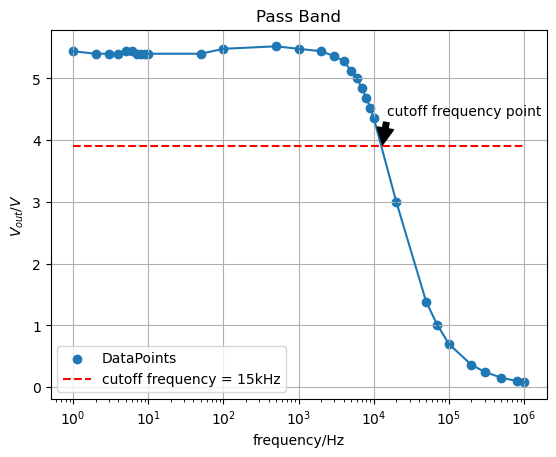
\includegraphics[width=0.5\textwidth]{ET2-2-1.png}
				\caption{差分放大器的通频带}
				\label{fig:ET2-2-1}
			\end{figure}
		
			所以其通频带约为 \textbf{0 - 15 kHz}。

	\end{enumerate}

	% % 讨论
	% \subsubsection{Discussion}
	% \begin{enumerate}
	% 	\item 
	% \end{enumerate}

	% 总结
	\subsubsection{Conclusion}
	\begin{itemize}
		\item 我们通过“先差分后放大”的思路,使用Model-D与Model-A串联使用,搭建了一个差分放大器,实现了最高103.56dB的共模抑制比。
		\item 同时,通过调节不同的反馈电阻的值,可以调整该放大器的放大倍数在 \textbf{0.048 - 404} 倍之间变化。
		\item 该差分放大器的通频带,经过测量,为\textbf{0 - 15kHz}。
	\end{itemize}


%---------------------------------------------------------------------
% 实验后思考题
% \subsection{Reflections after Experiment}

% %思考题1
% \begin{question}
	
% \end{question}

% % 思考题2
% \begin{question}
	
% \end{question}

% % 思考题3
% \begin{question}
	
% \end{question}
